\chapter{جداول التجزئة (\textenglish{Hash tables})}

للقوائم المتسلسلة نقطة ضعف كبيرة في حال أردنا قراءة محتواها : يستحيل الوصول إلى عنصر معيّن مباشرة. يجب التقدّم في القائمة عنصراً بعنصر حتى نجد العنصر الذي نريد. هذا يطرح مشاكل من ناحية الأداء ما إن يكون حجم القائمة المتسلسلة ضخماً. تخيّل قائمة متسلسلة تتكوّن من 1000 عنصر بينما العنصر الذي نبحث عنه موجود في آخرها !

تمثّل جداول التجزئة طريقة أخرى لتخزين البيانات. حيث أنها تستند على مبدأ الجداول في لغة الـ\textenglish{C}
و التي نعرف التعامل معها جيّداً. ماهي فائدتها الكُبرى ؟ هي تسمح بإيجاد سريع لعنصر محدد، سواء كان الجدول يحتوي 100، 1000، 10000 خانة أو حتى أكثر !

\section{لماذا نستعمل جدول تجزئة ؟}

لننطلق من المشكل الذي تطرحه القوائم المتسلسلة. هذه الأخيرة مرنة بشكل خاص، هذا ما استطعنا ملاحظته : يمكننا إضافة أو إزالة خانات في أي لحظة نريد، بينما يكون الجدول "ثابتاً" ما إن يتم إنشاؤه.

لكن، كما قلتُ لك في المقدّمة، للقوائم المتسلسلة عيب كبير : إذا أردنا استرجاع عنصر محدد من القائمة، يجب تصفّح هذه الأخيرة حتى نجد ذلك العنصر !

تخيّل قائمة متسلسلة تحتوي معلومات حول الطلّاب : الاسم، العُمر و المعدّل. سيتم تمثيل كلّ طالب بهيكل نسميه
\InlineCode{Student}.

\begin{information}
عملنا سابقاً على القوائم المتسلسلة التي تحتوي على
\InlineCode{int}.
 كما قلتُ لك، من الممكن تخزين أي شيء نريد في قائمة، حتى مؤشّراً نحو هيكل آخر كما سأقترحه لك الآن.
\end{information}

 إذا أردتُ الوصول إلى المعلومات الخاصة بالشخص
\textenglish{Luc Doncieux}
 في الصورة الموالية، يجب عليّ التقدّم في كلّ القائمة كي أكتشف بأنه العنصر الأخير فيها !
 
\begin{figure}[H]
	\centering
	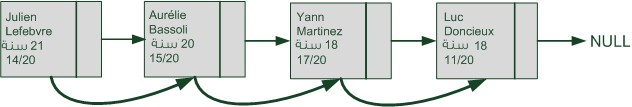
\includegraphics[width=0.8\textwidth]{Chapter_IV-3_Student-list}
\end{figure}

\begin{information}
بالفعل، لو أننا بحثنا عن الشخص 
\textenglish{Julien Lefebvre}،
كان البحث ليكون أسرع بما أنه متواجد في بداية القائمة. و مع ذلك، لتقييم كفاءة الخوارزمية، يجب أن نفكّر دائماً في أسوء الحالات. و الأسوء هو
\textenglish{Luc}
هنا.\\
هنا، نقول أن خوارزمية البحث لها تعقيد
(\textenglish{complexity})
\textit{\textenglish{O(n)}}،
لأنه يجب تصفّح كل القائمة المتسلسلة للوصول إلى العُنصر المراد، و في أسوء الحالات يكون هذا هو آخر عنصر. إذا كانت القائمة تحتوي على 9 عناصر، يجب أن يتم تشغيل 9 دورات للحلقة كحد أقصى لإيجاد العنصر.
\end{information}

في هذا المثال، لا تحتوي القائمة المتسلسلة سوى على أربعة عناصر. سيجد الحاسوب الشخص 
\textenglish{Luc Doncieux}
بسرعة كبيرة لا تسمح لنا حتى بأن نقول كلمة "أووه". لكن تخيّل أن هذا الشخص يتواجد في آخر قائمة متسلسلة من 10000 عنصر ! ليس مقبولا أن يتم البحث في 10000 عنصر لإيجاد المعلومة. هنا تتدخّل جداول التجزئة.

\section{ماهي جداول التجزئة ؟}

إذا كنت تتذكر جيداً، لا تعرف الجداول هذا النوع من المشاكل. لهذا، كي نصل إلى العنصر في الوضعية 2 من الجدول تكفيني كتابة التالي :

\begin{Csource}
int table[4] = {12, 7, 14, 33};
printf("%d", table[2]);
\end{Csource}

لو نعطي للحاسوب
\InlineCode{table[2]}،
فسيتوجّه مباشرة إلى المكان في الذاكرة أين هو مخزّن العدد 14. أي أنه لن يتقدّم في الجدول خانة بخانة.

\begin{question}
هل أنت بصدد القول أن الجداول ليست "بذلك القدر من السوء" ؟ لكن في هذه الحالة سنخسر الميزات التي توفّرها القوائم المتسلسلة التي تسمح لنا بإضافة و إزالة خانات في أي لحظة !
\end{question}

في الواقع، القوائم المتسلسلة مرنة أكثر. أما بالنسبة للجداول، فهي تسمح بالوصول السريع للمعطيات. يمكننا القول أن 
\textbf{جداول التجزئة}
تشكّل حلّا وسطا بين الإثنين.

يوجد عيب في استعمال الجداول لم نتكلّم عنه سابقاً : يتم تعريف خانات الجدول عن طريق أرقام نسمّيها 
\textbf{الفهارس}
(\textenglish{Indices}).
لا يمكن أن نطلب من الحاسوب : "ماهي المعلومات المتواجدة في الخانة التي تسمّى
"\textenglish{Luc Doncieux}".
أي أننا لإيجاد العُمر و المعدّل لن نتمكّن من كتابة :

\begin{Csource}
table["Luc Doncieux"];
\end{Csource}

مع أنه سيكون عملياً لو أننا نستطيع الوصول إلى خانة ما باستعمال الاسم فقط ! حسناً، هذا ممكن باستعمال جداول التجزئة.

\begin{information}
كما رأينا مؤخّراً. لا تشكّل جداول التجزئة "جزءً" من لغة الـ\textenglish{C}.
نتحدّث هنا عن مبدأ. سنعيد استعمال أساسيات لغة الـ\textenglish{C}
التي نعرفها من قبل لأجل إنشاء نظام ذكي جديد. و كأنه في لغة الـ\textenglish{C}،
باستعمال بعض الأدوات القاعدية، يمكننا إنشاء الكثير من الأشياء !
\end{information}

\begin{question}
بما أنه من الواجب أن يتم ترقيم الجدول بالفهارس، كيف سنجد رقم الخانة لو أننا نعرف الاسم
"\textenglish{Luc Doncieux}"
 فقط ؟
\end{question}

ملاحظة جيدة. في الواقع، يبقى الجدول جدولاً و لن يعمل إلا بالفهارس المرقّمة. تخيّل جدولاً يوافق الصورة الموالية : كل خانة لها فهرس و تتوفر على مؤشّر نحو هيكل من نوع
\InlineCode{Student}.
أنت تعرف القيام بهذا الآن :

\begin{figure}[H]
	\centering
	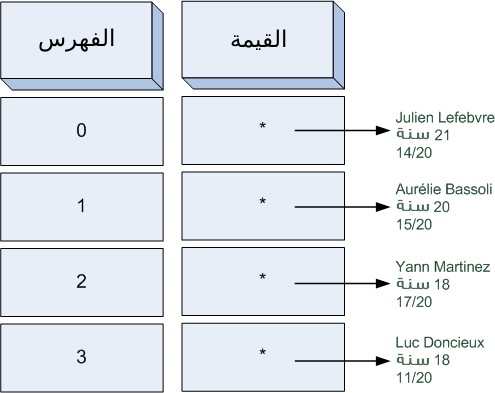
\includegraphics[height=0.3\textheight]{Chapter_IV-3_Array-indices}
\end{figure}

 لو أردنا إيجاد الخانة التي توافق
\textenglish{Luc Doncieux}،
 يجب أن نجيد تحويل الإسم إلى فهرس في الجدول. و بهذا، يجب أن نتمكّن من ربط كلّ اسم برقم من خانة في الجدول :

\begin{itemize}
	\item \textenglish{Julien Lefebvre} = $0$.
	\item \textenglish{Aurélie Bassoli} = $1$.
	\item \textenglish{Yann Martinez} = $2$.
	\item \textenglish{Luc Doncieux} = $3$.
\end{itemize}

لا يمكننا أن نكتب
\InlineCode{table["Luc Doncieux"]}
كما فعلتُ سابقاً. لأن هذا غير مسموح به في لغة الـ\textenglish{C}.

السؤال الذي يُطرح هو : كيف نحوّل سلسلة محارف إلى عدد ؟ هذا هو سحر التجزئة. تجب كتابة دالة تأخذ كمعامل سلسلة محارف، تطبّق حسابات عليها، ثم تُرجع لنا عدداً يوافق تلك السلسلة. سيكون هذا العدد هو فهرس الخانة في الجدول :

\begin{figure}[H]
	\centering
	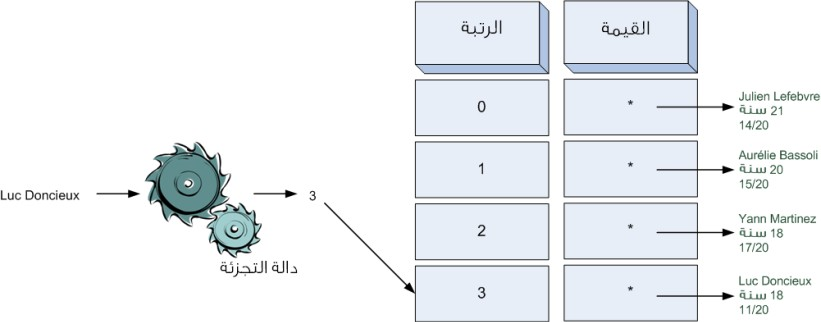
\includegraphics[width=\textwidth]{Chapter_IV-3_Array-indices-hash}
\end{figure}

\section{كتابة دالة تجزئة}

تكمن كلّ الصعوبة في كتابة دالة تجزئة صحيحة. كيف نحوّل سلسلةً محرفيّة إلى عدد وحيد ؟

أولا و قبل كلّ شيء، لنوضح الأمور : جدول التجزئة لا يحتوي 4 خانات كما أضع في الأمثلة، لكن 100 أو 1000 أو أكثر. لا يهم حجم الجدول، لأن البحث سيكون سريعاً جداً دائما.

\begin{information}
نقول أن هذا تعقيد بـدرجة
\textit{\textenglish{O(1)}}
لأننا نجد مباشرة عنصر البحث. في الواقع، دالة التجزئة سترجع لنا فهرسا : يكفي "القفز" مباشرة إلى الخانة الموافقة للجدول. لسنا بحاجة إلى تصفّح كلّ الخانات !
\end{information}

تخيّل إذاً جدولاً من 100 خانة، تقوم فيه بتخزين مؤشّرات نحو هياكل من نوع
\InlineCode{Student}.

\begin{Csource}
Student* table[100];
\end{Csource}

يجب علينا أن نكتب دالة، انطلاقاً من اسم، تولّد عدداً محصوراً بين 0 و 99 (رُتب الجدول). هنا يتطلّب منا الأمر الحذاقة. توجد طُرق رياضية جدّ معقّدة كي "نجزّء" البيانات، أي أن نحوّلها إلى أعداد.

\begin{information}
الخوارزميتان
\textenglish{MD5}
و
\textenglish{SHA1}
هما دالتا تجزئة مشهورتان، لكنهما متقدّمتان كثيرا بالنسبة لنا حالياً.
\end{information}

يمكنك اختراع دالة التجزئة الخاصة بك. هنا، لكي نبسّط الأمور، أقترح عليك ببساطة أن تجمع القيم
\textenglish{ASCII}
لكلّ حرف من الاسم، أي من أجل الاسم
\textenglish{Luc Doncieux}
ستكون لدينا عملية الجمع التالية :

\begin{Csource}
'L' + 'u' + 'c' + ' ' + 'D' + 'o' + 'n' + 'c' + 'i' + 'e' + 'u' + 'x'
\end{Csource}

سيكون لدينا مشكل : هذا المجموع يتخطّى الـ100 ! بما أن الجدول الذي أنشأناه لا يحتوي سوى على 100 خانة، فإن أخذنا بهذه القيمة فسنخاطر بالخروج من حدود الجدول.\\
أذكّرك بأن كلّ محرف في جدول
\textenglish{ASCII}
يمكن أن يكون مرقّما حتّى 255. و بهذا سنتجاوز بسرعة حاجز الـ100.

لحلّ هذا المشكل، يمكننا استعمال عامل الترديد
\InlineCode{\%}.
هل تتذكره ؟ إنّه يعطي باقي القسمة ! لو نقوم بهذا الحساب :

\begin{Csource}
lettersSum % 100
\end{Csource}

سنتحصّل قطعاً على عدد محصور بين 0 و 99. مثلاً، لو أن المجموع يساوي 4315، باقي القسمة على 100 هو 15. ستُرجع إذا دالة التجزئة القيمة 15.

إليك ما يمكن أن تكون عليه الدالة :

\begin{Csource}
int hash(char *string)
{
	int i = 0, hashNumber= 0;
	for (i = 0 ; string[i] != '\0' ; i++)
	{
		hashNumber += string[i];
	}
	hashNumber %= 100;
	return hashNumber;
}
\end{Csource}

لو نعطيها
\InlineCode{hash("Luc Doncieux")}،
ستُرجع لنا القيمة 55. و بـ\InlineCode{hash("Yann Martinez")}،
نتحصّل على 80.

بفضل دالة التجزئة هذه، يمكنك أن تعرف في أي خانة من الجدول يجب أن تضع المعلومات ! إذا أردت الوصول إلى هذه الخانات لاحقاً لاسترجاع المعلومة، تكفي "تجزئة" اسم الشخص من جديد لكي نجد فهرس الخانة في الجدول أين تخزّن المعلومات !

أنصحك بإنشاء دالة بحث تتكفّل بتجزئة المفتاح (الاسم) و تُرجع لنا مؤشّراً نحو المعلومات التي نبحثُ عنها. هذا سيعطينا مثلا :

\begin{Csource}
infoAboutLuc = findHashTable(table, "Luc Doncieux");
\end{Csource}

\section{معالجة التصادمات (\textenglish{Collisions management})}

حينما تُرجع دالة التجزئة نفس العدد من أجل مفتاحين مختلفين، نقول أنّه حدث 
\textbf{تصادم}.
مثلا في دالتنا، لو أننا نملك شخصاً اسمه تحريك أحرف لـ\textenglish{Luc Doncieux}،
مثلاً
\textenglish{Luc Doncueix}،
سيكون مجموع الأحرف هو نفسه، و بهذا فإن نتيجة دالة التجزئة ستكون نفسها !

يمكن لسببين أن يشرحا التصادم :

\begin{itemize}
	\item دالة التجزئة لا تعمل بكفاءة عالية. هذا يمثّل حالتنا. لقد كتبنا دالة سهلة جداً (لكن نوعاً ما كافية) من أجل الأمثلة. الدالتان 
	\textenglish{MD5}
	و
	\textenglish{SHA1}
	المذكورتان أعلاه هما ذات جودة عالية لأنهما تنتجان نسبة قليلة من التصادُمات. و لتعلم أن 
	\textenglish{SHA1}
	مفضّلة في أيامنا هذه أكثر من
	\textenglish{MD5}
	لأنها تننج نسبة تصادمات أقل مقارنة بنظيرتها.
	
	\item الجدول الذي نخزن به المعلومات صغير الحجم كثيراً. لو أننا ننشئ جدولا من 4 خانات و نريد تخزين 5 أشخاص، فسيحدث تصادم بالتأكيد، أي ان دالة التجزئة ستُعطي نفس الفهرس من أجل اسمين مختلفين.
\end{itemize}

إذا حصل تصادم فلا داعي للخوف ! هناك حلان يمكنك الاختيار بينهما : العـَنوَنـَة المفتوحة و السَلْسَلَة.


\subsection{العنونة المفتوحة (\textenglish{Open addressing})}
إذا بقيت أمكنة شاغرة في الجدول، يمكنك تطبيق التقنية التي تُدعى 
\textbf{التجزئة الخطيّة}.
المبدأ سهل. هل الخانة محجوزة ؟ لا يوجد مشكل، سننتقل للخانة التي تليها. آه، هل هذه محجوزة أيضاً ؟ توجّه لللتي بعدها.

و هكذا حتى تجد خانة موالية فارغة. إن وصلت إلى نهاية الجدول، فعد إلى البداية و أكمل البحث.

تطبيق هذه الطريقة سهل جداً، لكن إن واجهت الكثير من التصادمات، فسيكون عليك استغراق وقت كبير في البحث عن الخانة الشاغرة الموالية.

توجد طرق بديلة (التجزئة المزدوجة، التجزئة الرباعية \dots) و التي تنصّ على التجزّئة من جديد حسب دالة أخرى في حالة وجود تصادم. هذه الدوال أكثر كفاءة لكن أكثر تعقيدا من ناحية التطبيق.

\subsection{السَلْسَلَة (\textenglish{Chaining})}

حلّ آخر ينصّ على إنشاء قائمة متسلسلة في مكان التصادم. هل تريد تخزين بيانتين (أو أكثر) في نفس الخانة ؟ استعمل قائمة متسلسلة و أنشئ مؤشّراً نحو هذه القائمة انطلاقاً من الجدول :

\begin{figure}[H]
	\centering
	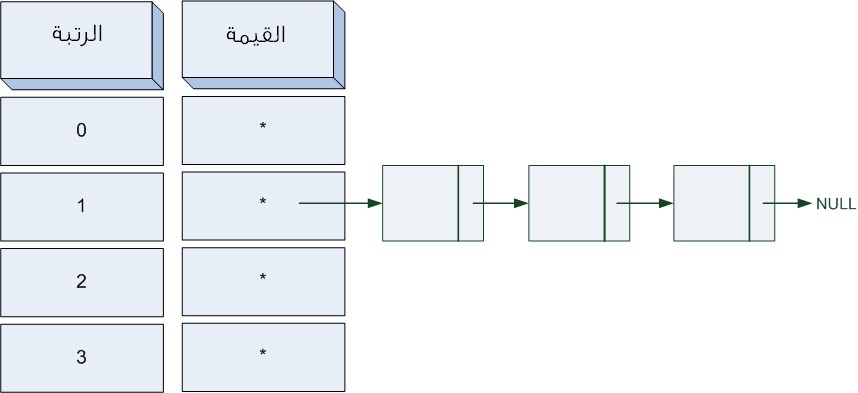
\includegraphics[height=0.3\textheight]{Chapter_IV-3_Hash-list}
\end{figure}

بالفعل، سنعود لمشكل القوائم المتسلسلة : إذا كان هناك 300 عنصرٍ في هذا الموقع من الجدول، يجب تصفّح القائمة المتسلسلة إلى حين إيجاد العنصر الصحيح.

هنا، كما ترى. ليست القوائم المتسلسلة دائماً الأمثل، لكن لجداول التجزئة حدودها أيضاً. يمكننا المزج بين الاثنين من أجل الحصول على الجانب الأفضل من كلّ بنية.

على أية حال، النقطة الحساسة في جداول التجزئة هي دالة التجزئة. فكلّما أنتجت تصادُمات أقل. كلما كان ذلك أفضل.
سأترك لك مهمة إيجاد دالة التجزئة المناسبة لحالتنا !

\section*{ملخّص}

\begin{itemize}
	\item القوائم المتسلسلة مرنة، لكن عملية إيجاد عنصر محدد تستغرق وقتاً طويلاً لأنه يجب تصفّح القائمة عنصراً بعنصر.
	\item جداول التجزئة هي جداول نخزّن فيها المعلومات في مكان محدد بواسطة دالة التجزئة.
	\item تأخذ دالة التجزئة مفتاحاً كمعامل (مثلاً : سلسلة محرفيّة) و تعيد عددا كمخرج.
	\item يتم استعمال هذا العدد لمعرفة عند أي فهرس من الجدول يجب تخزين البيانات.
	\item دالة التجزئة الأكثر كفاءة هي التي لا تولّد عدداً كبيراً من التصادُمات، أي أنها تتجنب قدر المستطاع إرجاع نفس العدد من أجل مفتاحين مختلفين.
	\item في حالة التصادم، يمكننا استعمال تقنية العنونة المفتوحة (البحث عن خانة شاغرة أخرى في الجدول) أو استعمال تقنية السلسلة (الدمج مع القوائم المتسلسلة).
\end{itemize}
